\chapter{Comunicando Paramics con OMNeT++ mediante TraCI}
\section{Diseño Arquitectural}\label{sec:architecture}

El software desarrollado consiste en un \emph{plugin} que extiende la funcionalidad de Paramics, agregándole la capacidad de comportarse como un servidor TraCI. Específicamente, el \emph{plugin} consiste en una implementación parcial de un servidor TraCI, el cual se ejecuta en un \emph{thread} paralelo a Paramics; este se encuentra a su vez simulando en modo discreto, esperando instrucciones para avanzar la simulación. La comunicación entre ambos se efectúa a través de la API de extensión de Paramics.

La figura \ref{fig:ptraci_arch} ilustra esta arquitectura. A pesar de que se encuentra implementado como un \emph{plugin} de Paramics, el servidor TraCI es prácticamente un programa independiente, y su interacción con el simulador de transporte se limita a un conjunto acotado de llamados a su API.

\begin{figure}[t]
    \centering
    \begin{sequencediagram}
    \newthread{D}{OMNeT++}{}
    \newinst[1]{A}{VEINS}{}
    \newinst[3]{B}{Plugin}{}
    \newthread[3]{C}{Paramics}{}
    
    \begin{messcall}{C}{run()}{B}
        \postlevel
        \begin{call}{B}{waitForCommands()}{B}{}
        \end{call}
    \end{messcall}
    
    \begin{call}{D}{Solicitud}{A}{Resultado}
    
        \begin{call}{A}{Comando TraCI}{B}{Respuesta TraCI}
            \begin{call}{B}{parseCommand()}{B}{sendResponse()}
                \postlevel
                \begin{call}{B}{API Paramics}{C}{Datos}
                \end{call}
                \postlevel
            \end{call}
        \end{call}
    \end{call}
\end{sequencediagram}
    \caption{Arquitectura del Framework}
    \label{fig:ptraci_arch}
\end{figure}

Describir separación de archivos, namespaces.

\section{Módulos Principales}
\subsection{plugin.c}

Si bien en estricto rigor no es un módulo del \emph{framework}, merece ser mencionado al ser el archivo principal del \emph{plugin} desarrollado. En este archivo se definen las funciones de extensión (prefijo \texttt{QPX}, ver sección \ref{sec:paramics_api}) a ser invocadas por Paramics al inicializar el \emph{plugin}. A continuación se describirán brevemente las más importantes de estas funciones, mientras que el archivo \texttt{plugin.c} puede estudiarse en su totalidad en el código \ref{code:pluginc} en los anexos.

\subsubsection{\texttt{void qpx\_NET\_postOpen(void)}}\label{sec:qpx_postopen}

Invocada inmediatamente luego de que Paramics carga la red y el \emph{plugin}, esta función cambia el modo de ejecución de Paramics a su modo discreto e inicializa el servidor TraCI. Para esto, crea un \emph{thread} donde corre una función auxiliar \texttt{runner\_fn()}, la cual se encarga de:

\begin{enumerate}
    \item Obtener el puerto en el cual esperar conexiones entrantes desde los parámetros de ejecución de Paramics. De no haberse especificado puerto, utiliza uno por defecto.
    \item Inicializar un objeto \emph{TraCIServer} (ver sección \ref{sec:traciserver}) encargado de las conexiones entrantes en el puerto anteriormente definido.
\end{enumerate}

\subsubsection{\texttt{void qpx\_VHC\_release(VEHICLE* vehicle)}}

Función invocada por Paramics cada vez que un vehículo es liberado a la red de transporte. Simplemente se encarga de notificar al \emph{VehicleManager} (ver sección \ref{sec:vehiclemanager}) para su inclusión en el modelo interno del \emph{plugin}.

\subsubsection{\texttt{void qpx\_VHC\_arrive(VEHICLE* vehicle, LINK* link, ZONE* zone)}}

Invocada cuando un vehículo alcanza su destino final, esta función notifica al \emph{VehicleManager} para eliminar el vehículo en cuestión de la representación interna.

\subsection{TraCIServer}\label{sec:traciserver}

Implementa el funcionamiento base del servidor TraCI. Es el primer módulo como tal en inicializarse, y tiene como funciones:

\begin{enumerate}
    \item Asociarse a un \emph{socket} TCP, y esperar una conexión de un cliente TraCI.
    \item Mientras exista una conexión abierta, recibir e interpretar comandos TraCI entrantes.
    \begin{itemize}
        \item En el caso de los comandos de obtención de versión y cierre de la conexión, estos son ejecutados por el módulo mismo.
        \item El comando de avance de simulación es ejecutado parcialmente por este módulo y el módulo \emph{Simulation} (ver sección \ref{sec:simulation}). Específicamente, se delega el avance del estado de la simulación a \emph{Simulation}, luego del cual se realiza la evaluación de las suscripciones en \emph{TraCIServer}.
        \item Demás comandos son delegados a los módulos pertinentes.
    \end{itemize}
    \item Escribir mensajes de estado y respuesta a comandos TraCI.
    \item Al recibir un comando de cierre, finalizar la simulación y cerrar el \emph{socket}.
\end{enumerate}

El módulo en cuestión se implementó como una clase de C++ en los archivos \texttt{src/TraCIAPI/TraCIServer.h} y \texttt{src/TraCIAPI/TraCIServer.cpp}, y se instancia en el archivo \texttt{plugin.c}. Se implementó considerando que se ejecutaría en un \emph{thread} paralelo al principal de Paramics, y por lo tanto incluye elementos de sincronización.

Cabe destacar que para facilitar el uso de \emph{sockets} y la obtención y envío de datos a través de éstos, se utilizaron las clases \texttt{tcpip::Socket} y \texttt{tcpip::Storage}, definidas en los archivos \texttt{src/shawn/socket.\{cpp/h\}} y \texttt{src/shawn/storage.\{cpp/h\}}. \texttt{tcpip::Socket} abstrae el funcionamiento de un \textit{socket} TCP, y provee métodos de conveniencia que permiten leer y escribir mensajes TraCI completos como objetos \texttt{tcpip::Storage}. Estos a su vez proveen métodos para escribir y leer todo tipo de variables en dichos mensajes, sin la necesidad de hacer la conversión manual a \textit{bytes}.

Estos archivos no fueron desarrollados por el memorista, sino que fueron obtenidos desde el código fuente de SUMO \footnote{Fuente SUMO: \url{https://github.com/planetsumo/sumo/tree/master/sumo/src/foreign/tcpip}. Debe notarse que, a su vez, los creadores de SUMO originalmente obtuvieron dichos archivos del código fuente del simulador de eventos discretos para redes de sensores \emph{SHAWN} \cite{kroller2005shawn}. Su fuente original se encuentra en \url{https://github.com/itm/shawn/tree/master/src/apps/tcpip}}, distribuidos bajo una licencia BSD\footnote{Licencia clases \texttt{tcpip::Socket} y \texttt{tcpip::Storage}: \url{http://sumo.dlr.de/wiki/Libraries_Licenses\#tcpip_-_TCP.2FIP_Socket_Class_to_communicate_with_other_programs}}.

A continuación se detalla la implementación de las funcionalidades anteriormente mencionadas.

\subsubsection{Inicio de conexión TraCI}

Como se mencionó en la sección \ref{sec:qpx_postopen}, al iniciarse el \emph{plugin} se crea un nuevo \emph{thread}, en el cual se instancia un objeto de la clase \texttt{TraCIServer}, al cual se le invoca su método \texttt{run()} (código \ref{cod:traciserver_run}).

\lstinputlisting[float=t, style=CPP, label={cod:traciserver_run}, caption={Rutina de inicio de conexión.}]{codigo/traciserver_run.cpp}
%\minipagelisting{codigo/traciserver_run.cpp}{Rutina de inicio de conexión.}{cod:traciserver_run}

Este método es simple: imprime información pertinente sobre el \emph{plugin} en la ventana de información de Paramics, y luego procede a bloquear el \emph{thread} mientras espera una conexión entrante en el \emph{socket}. Al recibirla, resume la ejecución y realiza un llamado al método \texttt{waitForCommands()} para comenzar a recibir e interpretar comandos TraCI.

\subsubsection{Recepción e Interpretación de Comandos Entrantes}

El método \texttt{waitForCommands()}, presentado en el código \ref{cod:traciserver_waitforcommands}, se encarga de recibir mensajes TraCI entrantes y separar los comandos para su posterior interpretación.

El código inicia un \emph{loop} dentro del cual monitorea el \emph{socket}. Al recibir datos entrantes, el \emph{socket} retorna un objeto \texttt{tcpip::Storage} con el mensaje completo. Luego, en un \emph{loop} adicional, este mensaje se separa en sus comandos TraCI constituyentes, copiando la información perteneciente a cada comando en otro objeto \texttt{tcpip::Storage} temporal. Este objeto se entrega como parámetro al método \texttt{parseCommand()} para la interpretación del comando, luego de lo cual se limpia y se vuelve a utilizar para el siguiente comando.

Finalmente, interpretados todos los comandos, se envía la respuesta al cliente a través del mismo \emph{socket} y se limpian los objetos \texttt{tcpip::Storage} para su reutilización en una nueva iteración del \emph{loop}.

\lstinputlisting[style=CPP, label={cod:traciserver_waitforcommands}, caption={Recepción de mensajes desde el \emph{socket} TCP.}]{codigo/traciserver_waitforcommands.cpp}
%\minipagelisting{codigo/traciserver_waitforcommands.cpp}{Recepción de mensajes desde el \emph{socket} TCP.}{cod:traciserver_waitforcommands}

Como se mencionó anteriormente, la interpretación de los comandos se lleva a cabo en el método \texttt{parseCommand()}, el cual recibe un único comando encapsulado en un objeto \texttt{tcpip::Storage}. Este método tiene una única misión; interpretar el identificador del comando recibido y delegar su ejecución al método correspondiente de la clase \texttt{TraCIServer}. Su implementación es simple, aunque un poco tediosa, y su esqueleto puede observarse en el código \ref{cod:traciserver_parsecommand}. En específico, el código del método se puede dividir en dos ramas de ejecución; en caso de comando de suscripción (cuyos identificadores se encuentran todos en el rango $[\texttt{0xd0}, \texttt{0xdb}]$) se extraen los parámetros de la suscripción y se invoca el método \texttt{addSubscription()} para la subsecuente validación y activación de ésta. Por el contrario, en case de recibir un comando con identificador fuera de dicho rango, se procede a verificar su tipo mediante un \emph{switch}. Cada caso se relaciona con un comando y método específico a invocar, y en caso de no encontrarse el identificador en cuestión se notifica al cliente que el comando deseado no está implementado.

\lstinputlisting[style=CPP, label={cod:traciserver_parsecommand}, caption={Esqueleto de \texttt{parseCommand()}}]{codigo/traciserver_parsecommand.cpp}

\subsubsection{Avance de Simulación y Evaluación de Suscripciones}

En caso de recibir un comando de avance de simulación, \emph{TraCIServer} delega la ejecución de dicho avance al módulo \emph{Simulation}. Sin embargo, al terminar este procedimiento, se realiza la evaluación de las suscripciones activas en \emph{TraCIServer}, mediante el método \texttt{processSubscriptions()}.

Como se detalló en la sección \ref{sec:traci}, el protocolo TraCI define 12 tipos de suscripciones a variables de objeto, las cuales comparten todas una estructura idéntica. Cada suscripción se caracteriza por su identificador de tipo y sus parámetros: tiempo de inicio, tiempo de fin, identificador del objeto y las variables a las cuales el cliente se ha suscrito. En la práctica, lo único que diferencia a las suscripciones entre sí son las categorías de objetos a las cuales están asociadas, y por ende, cómo obtener esos datos desde la implementación interna del \emph{plugin}. A raíz de esto, se decidió implementar un árbol de clases de C++ para representar las suscripciones en memoria (declarada e implementada en los archivos \texttt{src/TraCIAPI/Subscriptions.h} y \texttt{src/TraCIAPI/Subscriptions.cpp} respectivamente).

La raíz de éste árbol, la clase \texttt{VariableSuscription}, implementa la funcionalidad completa de evaluación y actualización de una suscripción, abstrayendo la obtención de datos específicos a cada tipo en los métodos \texttt{getObjectVariable()} y \texttt{getResponseCode()}. Estos métodos son \emph{virtuales} en la clase base, y son implementados por las clases derivadas, de manera que \emph{TraCIServer} sólo necesita mantener un vector de variables del tipo base, las cuales se evalúan de manera polimórfica.

En términos más simples, lo único que diferencia a las diferentes clases de suscripciones en la implementación son los métodos \texttt{getObjectVariable()} y \texttt{getResponseCode()} anteriormente mencionados. Para dar un ejemplo, para suscripciones de variables de vehículos, estos métodos se ven así:

\lstinputlisting[style=CPP, label={cod:vehiclesub}, caption={Ejemplo de métodos extendidos en \emph{VehicleVariableSubscription}}]{codigo/vehiclesub.cpp}
%\minipagelisting{codigo/vehiclesub.cpp}{Ejemplo de métodos extendidos en \emph{VehicleVariableSubscription}}{cod:vehiclesub}
    
%\begin{figure}
%    \centering
%    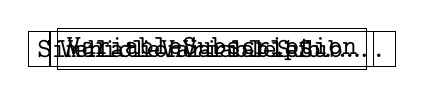
\begin{tikzpicture}
\tikzset{level distance=50pt}
\Tree [.\node[draw]{\texttt{VariableSubscription}};
[.\node[draw]{\texttt{VehicleVariableSub\dots}}; ]
[.\node[draw]{\texttt{SimulationVariableSub\dots}}; ]
[.{\dots} ]
]
\end{tikzpicture}
%    \caption{Árbol de herencia de suscripciones.}
%    \label{fig:subs_tree}
%\end{figure}

\subsection{Simulation}\label{sec:simulation}
\subsection{VehicleManager}\label{sec:vehiclemanager}